\documentclass{article}

\usepackage{graphicx}


\title{RDFtex: Import and Export Examples}
\date{}


\usepackage[export]{adjustbox}
\begin{document}
\maketitle

\section{Imported Contributions}

\subsection*{Definition Import}

\subsection*{Dataset Import}

\subsection*{Figure Import}


\begin{figure}[htb!]
\centering
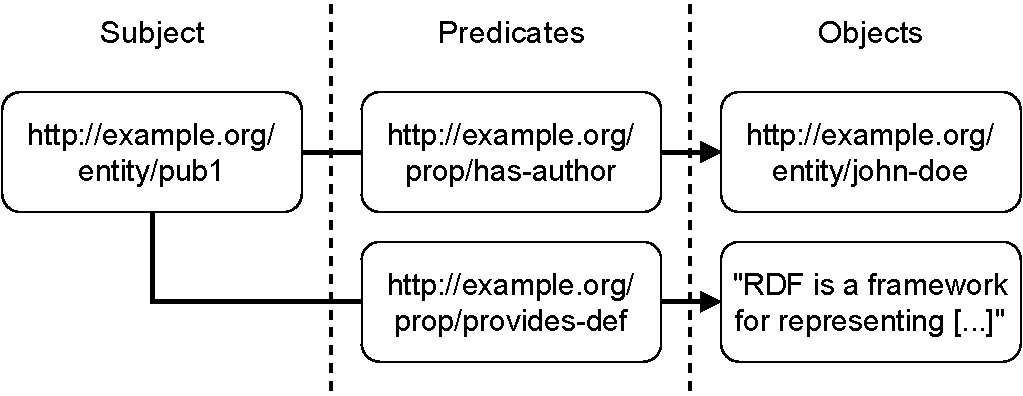
\includegraphics[max width=0.7\columnwidth]{./figures/triple_example}
\caption{A simple exemplary knowledge graph consisting of two RDF triples. The upper triple provides contextual information, the lower triple contentual information of the publication \emph{{pub1}}. All non-literal triple members are identified using IRIs. (Figure and caption adopted from~\cite{Martin21}.)}
\label{fig:contentual-contextual}
\end{figure}

\subsection*{Experimental Result Import}

\subsection*{Software Import}

\section{Export}

\subsection*{Definition Export}

\subsection*{Dataset Export}

\subsection*{Figure Export}

\subsection*{Experimental Result Export}

\subsection*{Software Export}

\bibliographystyle{plain}
\bibliography{example}

\end{document}